\section{Auswertung}
\label{sec:Auswertung}
\subsection{Die mittlere freie Weglänge}
Die mittlere freie Weglänge $\bar{w}$ wurde nach \eqref{eqn:freieweglaengetheorie} aus den Temperaturen berechnet.
Die dafür benötigte Berechnung des Sättigungsdampfdruckes wurde nach \eqref{eqn:sättigungsdampfdrtheorie} durchgeführt.
In folgender Tabelle sind die Weglängen für die verschiedenen Temperaturen aufgeführt.

\begin{table}[H]
  \centering
    \caption{Die mittlere freie Weglänge für verschiedene Temperaturen.}
    \label{tab:freieweglaengeausw}
    \sisetup{table-format=3.2}
      \begin{tabular}{S S[table-format=2.3] S[table-format=2.3] S[table-format=2.3]}
        \toprule
        {Temperatur [$\si{\kelvin}$]} & {$p_\text{Sätt}$}  & {$\bar{w}$ [$\si{\milli\bar}$]} & {$\frac{a}{\bar{w}}$} \\
        \midrule
         297.15  &    \num{4.908e-03}      &          0.591  &  \num{1.692e-2} \\
         417.05  &              3.802      & \num{7.627e-4}  &          13.111 \\
         447.25  &             11.576      & \num{2.505e-4}  &          39.916 \\
         471.15  &             25.248      & \num{1.149e-4}  &          87.064 \\
        \bottomrule
      \end{tabular}
    \end{table}
\noindent
\subsection{Die differentielle Energieverteilung der Elektronen}
Um die differentielle Energieverteilung der Elektronen zu erhalten, muss zuerst die Skalierung ermittelt werden.
Dafür wurde die Spannung bei $\SI{0}{\volt}, \SI{1}{\volt}, ..., \SI{10}{\volt}$ auf der Abzisse eingezeichnet.
Aus der Breite dieser $\SI{1}{\volt}$-Abstände wird der Mittelwert gebildet, um eine Relation zwischen
$\si{\milli\meter}$ und $\si{\volt}$ zu erhalten. Dies wurde für die beiden Messreihen durchgeführt und ist in
folgender Tabelle zusammengefasst.

\begin{table}[H]
  \centering
  \caption{Die Skalierung der beiden Messreihen.}
  \label{tab:skalierungausw}
  \sisetup{table-format=2.2}
    \begin{tabular}{S S S}
      \toprule
      {Abschnitt [$\si{\volt}$]} & {Breite Messreihe 1 [$\si{\milli\meter}$]} & {Breite Messreihe 2 [$\si{\milli\meter}$]} \\
      \midrule
      {0-1}  &  23   & 25.5  \\
      {1-2}  &  22   & 22  \\
      {2-3}  &  22.5 & 23  \\
      {3-4}  &  23.5 & 21.5  \\
      {4-5}  &  23   & 24  \\
      {5-6}  &  23   & 24  \\
      {6-7}  &  23.5 & 24  \\
      {7-8}  &  24   & 24  \\
      {8-9}  &  23.5 & 23  \\
      {9-10} &  25   & 26  \\
      {$\rightarrow$} & \num{23.3 \pm 0.260} mm/V  & \num{23.7 \pm 0.442} mm/V \\
      \bottomrule
    \end{tabular}
  \end{table}
\noindent
In der letzten Zeile der Tabelle sind die Mittelwerte aufgeführt. Da auf der Skala maximal im
$\si{\milli\meter}$-Bereich genau Werte abgelesen
werden können, werden im Folgenden die Unsicherheiten der Mittelwerte vernachlässigt, da nicht sicher
zwischen Unsicherheit und Ablesegenauigkeit unterschieden werden kann.
Um die differentielle Energieverteilung zu erhalten, werden an den Graphen
Steigungsdreiecke angelegt. Dies ist in Abbildung \ref{fig:} zu erkennen.
Die differentiellen Energieverteilungen sind in folgenden Tabellen dargestellt.


\begin{table}[H]
  \centering
  \caption{Die differentielle Energieverteilung der zwei Messreihen im Durchgang 1.}
  \label{tab:diffenergiev1}
  \sisetup{table-format=2.2}
    \begin{tabular}{S S S S}
      \toprule
      \multicolumn{2}{c}{Messreihe 1 ($\SI{24}{\celsius}$)} & \multicolumn{2}{c}{Messreihe 2 ($\SI{143.9}{\celsius}$) } \\
      \cmidrule(lr){1-2}\cmidrule(lr){3-4}
      {Position $x$ [$\si{\milli\meter}$]} & {Steigung $\frac{\increment y}{\increment x}$ } &
      {Position $x$ [$\si{\milli\meter}$]} & {Steigung $\frac{\increment y}{\increment x}$ } \\
      \midrule
      {0-10}    & 0   & {0-10}    & 1.1 \\
      {10-20}   & 0   & {10-20}   & 1.2 \\
      {20-30}   & 0   & {20-30}   & 1.1 \\
      {30-40}   & 0   & {30-40}   & 1.2 \\
      {40-50}   & 0.1 & {40-50}   & 1.2 \\
      {50-60}   & 0.1 & {50-60}   & 1.1 \\
      {60-70}   & 0.1 & {60-70}   & 1.1 \\
      {70-80}   & 0.1 & {70-80}   & 1.1 \\
      {80-90}   & 0.1 & {80-90}   & 1   \\
      {90-100}  & 0.1 & {90-100}  & 0.6 \\
      {100-110} & 0.1 & {100-100} & 0.3 \\
      {110-120} & 0.1 & {110-120} & 0   \\
      {120-130} & 0.2 & {120-130} & 0.1 \\
      {130-140} & 0.2 & {130-140} & 0.1 \\
      {140-150} & 0.2 & {140-150} & 0.1 \\
      {150-160} & 0.2 & {150-160} & 0.1 \\
      {160-170} & 0.3 & {160-170} & 0.1 \\
      {170-180} & 0.4 & {170-180} & 0.1 \\
      {180-190} & 0.7 & {180-190} & 0.2 \\
      {190-200} & 1.6 & {190-200} & 0.2 \\
      {200-210} & 6.9 & {200-210} & 0.1 \\
      {210-220} & 0.9 & {210-220} & 0.1 \\
      {220-230} & 0   & {220-230} & 0.1 \\
      {230-240} & 0   & {230-240} & 0   \\
      {240-250} & 0   & {240-250} & 0   \\
      \bottomrule
    \end{tabular}
  \end{table}

\begin{table}[H]
  \centering
  \caption{Die differentielle Energieverteilung der zwei Messreihen im Durchgang 2.}
  \label{tab:diffenergiev2}
  \sisetup{table-format=2.2}
    \begin{tabular}{S S S S}
      \toprule
      \multicolumn{2}{c}{Messreihe 1 ($\SI{24}{\celsius}$)} & \multicolumn{2}{c}{Messreihe 2
      ($\SI{143.9}{\celsius}$) } \\
      \cmidrule(lr){1-2}\cmidrule(lr){3-4}
      {Position $x$ [$\si{\milli\meter}$]} & {Steigung $\frac{\increment y}{\increment x}$ } &
      {Position $x$ [$\si{\milli\meter}$]} & {Steigung $\frac{\increment y}{\increment x}$ } \\
      \midrule
      {0-10}    & 0   & {0-10}    & 1.3 \\
      {10-20}   & 0   & {10-20}   & 1.2 \\
      {20-30}   & 0   & {20-30}   & 1.2 \\
      {30-40}   & 0   & {30-40}   & 1.2 \\
      {40-50}   & 0   & {40-50}   & 1.2 \\
      {50-60}   & 0   & {50-60}   & 1.1 \\
      {60-70}   & 0.1 & {60-70}   & 1.1 \\
      {70-80}   & 0.1 & {70-80}   & 1.1 \\
      {80-90}   & 0.1 & {80-90}   & 1.1 \\
      {90-100}  & 0.1 & {90-100}  & 0.8 \\
      {100-110} & 0.1 & {100-100} & 0.3 \\
      {110-120} & 0.1 & {110-120} & 0.1 \\
      {120-130} & 0.1 & {120-130} & 0.1 \\
      {130-140} & 0.2 & {130-140} & 0.1 \\
      {140-150} & 0.2 & {140-150} & 0.1 \\
      {150-160} & 0.3 & {150-160} & 0.1 \\
      {160-170} & 0.4 & {160-170} & 0.1 \\
      {170-180} & 0.5 & {170-180} & 0.1 \\
      {180-190} & 0.8 & {180-190} & 0.1 \\
      {190-200} & 1.6 & {190-200} & 0.1 \\
      {200-210} & 6.8 & {200-210} & 0.1 \\
      {210-220} & 0.8 & {210-220} & 0.1 \\
      {220-230} & 0.1 & {220-230} & 0.1 \\
      {230-240} & 0   & {230-240} & 0   \\
      {240-250} & 0   & {240-250} & 0   \\
      \bottomrule
    \end{tabular}
  \end{table}

Die differentielle Energieverteilung ist in folgenden Plots grafisch dargestellt.

\begin{figure}[H]
  \centering
  \includegraphics[scale=0.7]{auswertung/differentielleEnergie1.pdf}
  \caption{Die differentielle Energieverteilung für zwei Temperaturen im ersten Messdurchgang.}
  \label{fig:diffenergie1}
\end{figure}

\begin{figure}[H]
  \centering
  \includegraphics[scale=0.7]{auswertung/differentielleEnergie2.pdf}
  \caption{Die differentielle Energieverteilung für zwei Temperaturen im zweiten Messdurchgang.}
  \label{fig:diffenergie2}
\end{figure}
\noindent
An den Graphen ist gut erkennbar, dass der höchste Ansteig bei $9.012\si{\electronvolt}$
beziehungsweise bei $8.860\si{\electronvolt}$ liegt. Dies sind auch die Energien, die die meisten
Elektronen besitzen.
Nach der Theorie müsste der Peak eigentlich nur eine verschwindende Breite besitzen.
Das sich dies hier nicht zeigt, liegt an der Fermi-Dirac Statistik (siehe \ref{sec:fermidirac}).
Der Einfluss der Temperatur auf den Kurvenverlauf lässt sich so erklären, dass bei erhöhten
Temperaturen mehr Zusammenstöße der Elektronen mit dem Quecksilber entstehen.
Die beginnende Abwärtstendenz bei ca. $\SI{3}{\volt}$ rührt daher, dass dies genau die
Differenz aus der ersten Anregungsenergie (siehe \ref{sec:anrhgat}) und dem Kontaktpotential.
\noindent
Das Kontaktpotential ergibt sich nach \eqref{eqn:effpottheorie} zu
\begin{align}
  K_1  & = 11 \si{\volt} -  9.012 \si{\volt} = 1.988 \si{\volt} \\
  K_2  & = 11 \si{\volt} -  8.860 \si{\volt} = 2.14  \si{\volt}
  \label{eqn:kpotausw}
\end{align}
\noindent
wobei hier $K_1$ aus dem ersten Messdurchlauf und $K_2$ aus dem zweiten Messdurchlauf bestimmt wurde.
Die Graphen, welche die Basis für die Bestimmung der differentiellen Energieverteilung liefern, sind
im Folgenden abgebildet.
\begin{figure}[H]
  \centering
  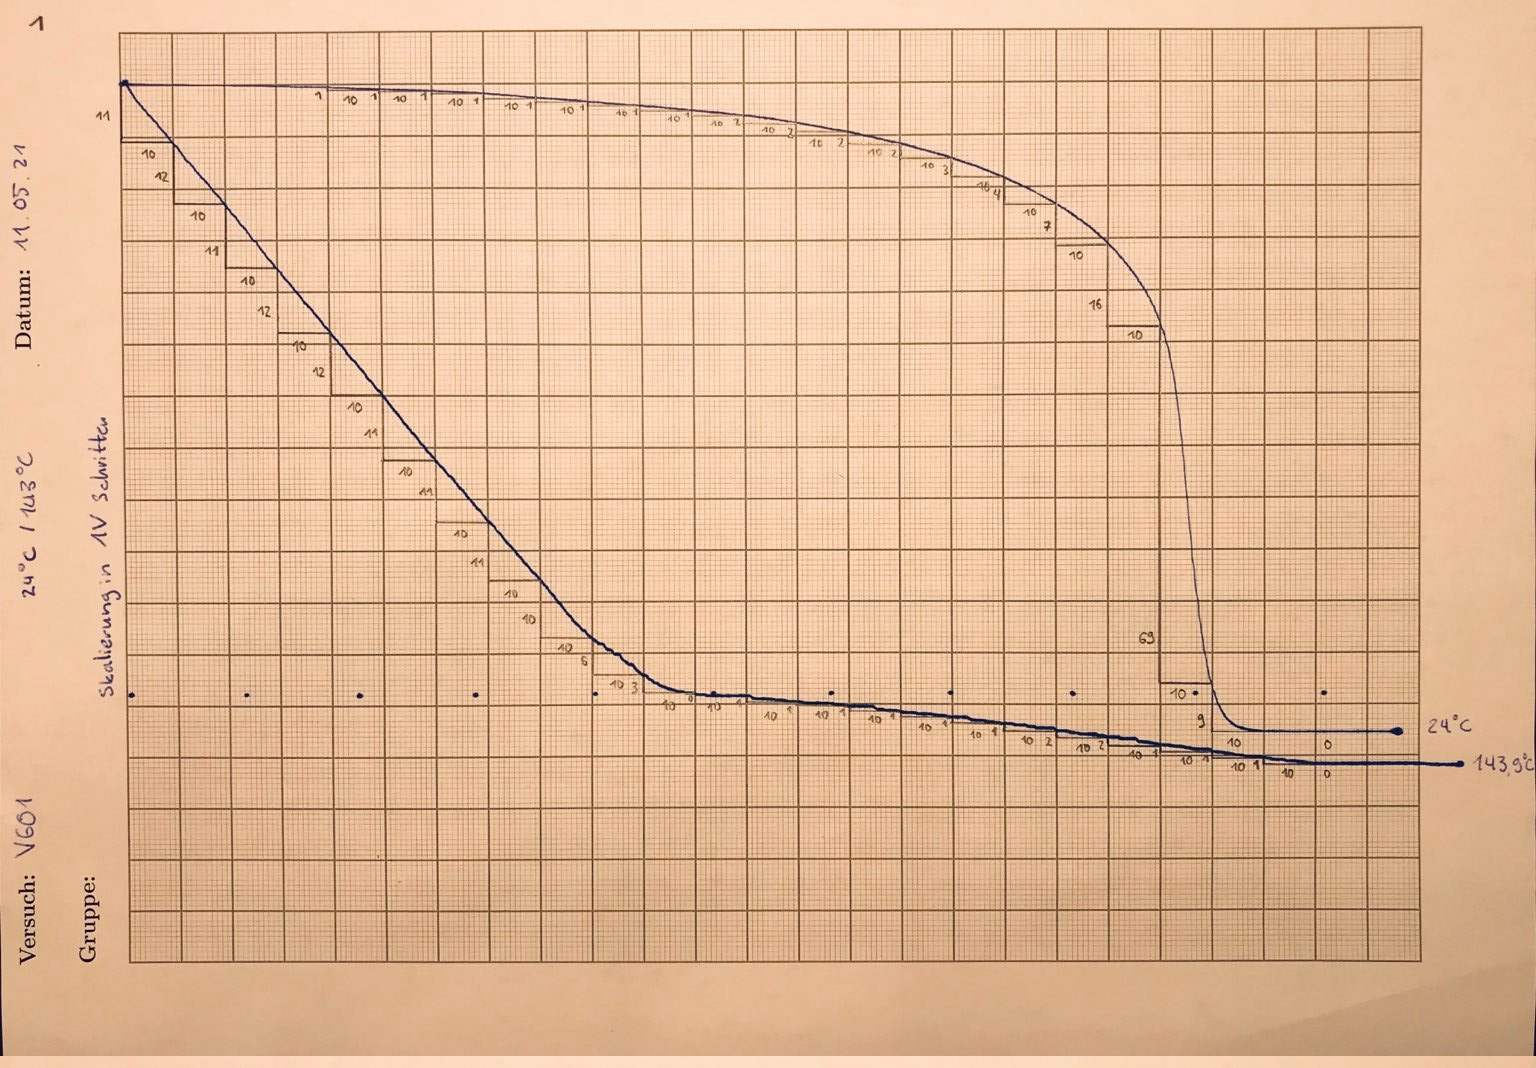
\includegraphics[scale=0.25]{content/kurve1.jpeg}
  \caption{Die Aufnahme der Energieverteilung bei verschiedenen Temperaturen aus dem ersten Messdurchgang.}
  \label{fig:franckhertz1}
\end{figure}
\begin{figure}[H]
  \centering
  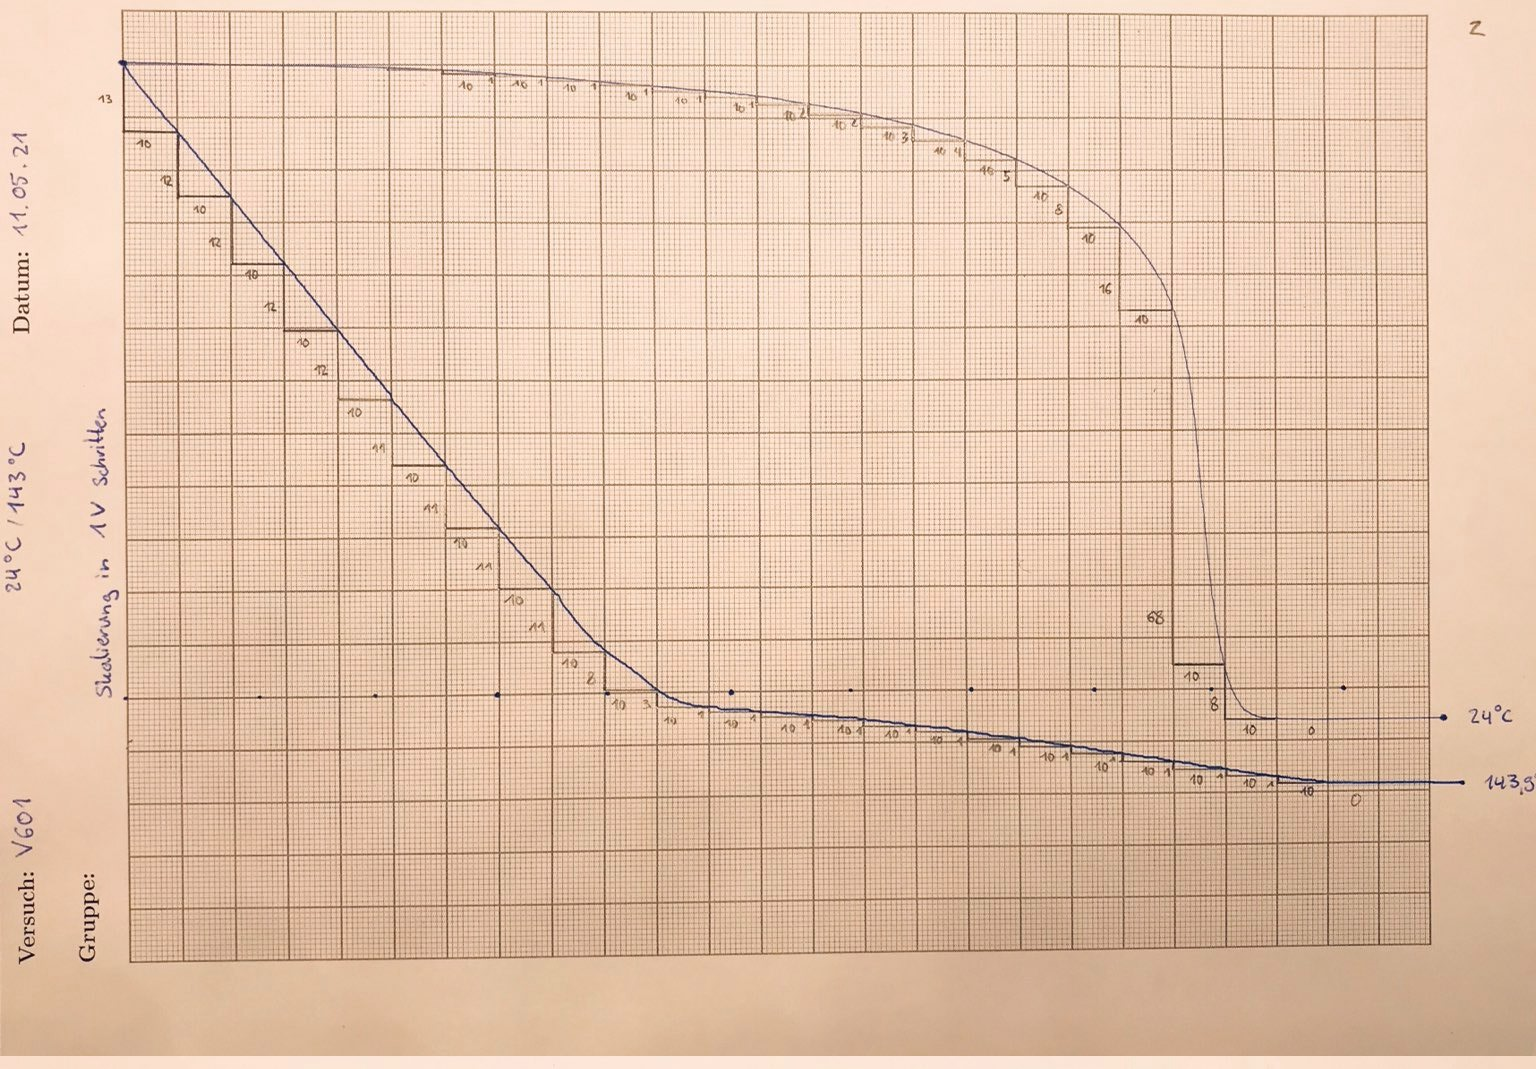
\includegraphics[scale=0.25]{content/kurv2.jpeg}
  \caption{Die Aufnahme der Energieverteilung bei verschiedenen Temperaturen im zweiten Messdurchgang.}
  \label{fig:franckhertz2}
\end{figure}

\subsection{Die Anregungsenergie des Hg-Atoms}
\label(sec:anrhgat)
Die Skalierung der aufgenommenen Franck-Hertz Kurven muss muss zuerst bestimmt werden
und ist in folgender Tabelle dargestellt.

\begin{table}[H]
  \centering
  \caption{Die Skalierung der beiden Messreihen.}
  \label{tab:skalierungauswfranckhertz}
  \sisetup{table-format=2.2}
    \begin{tabular}{S S S}
      \toprule
      {Abschnitt [$\si{\volt}$]} & {Breite Messreihe 1 [$\si{\milli\meter}$]} & {Breite Messreihe 2
      [$\si{\milli\meter}$]} \\
      \midrule
      {0-5}   &  18   & 22   \\
      {5-10}   &  21   & 21   \\
      {10-15}  &  21   & 20   \\
      {15-20}  &  21.5 & 22.5 \\
      {20-25}  &  20   & 18   \\
      {25-30}  &  20.5 & 21   \\
      {30-35}  &  21   & 21   \\
      {35-40}  &  21   & 19   \\
      {40-45}  &  20.5 & 19.5 \\
      {45-50}  &  21.5 & 21   \\
      {50-55}  &  23   & 14   \\
      {$\rightarrow$} & \num{20.818 \pm 0.365} mm/V  & \num{19.909 \pm 0.710} mm/V \\
      \bottomrule
    \end{tabular}
  \end{table}
\noindent
Da die Fehler wieder in der selben Größenordnung wie die Ablesegenauigkeit der Skala
liegen, werden sie vernachlässigt.
Zur Bestimmung der ersten Anregungsenergie werden die Abstände der Maxima der
Franck-Hertz Kurven aufgenommen und gemittelt. Dies ist in folgender Tabelle
wiedergegeben.

\begin{table}[H]
  \centering
  \caption{Die Abstände der Maxima der beiden Franck-Hertz Kurven.}
  \label{tab:skalierungauswfranckhertz}
  \sisetup{table-format=2.2}
    \begin{tabular}{S S S}
      \toprule
      {Maximum} & {Abstand Maxima Kurve 1 [$\si{\milli\meter}$]} & {Abstand Maxima Kurve 2
      [$\si{\milli\meter}$]} \\
      \midrule
      1  &  20   & 21   \\
      2  &  21.5 & 21   \\
      3  &  21   & 21   \\
      4  &  22.5 & 21   \\
      5  &  18   & 21   \\
      6  &  24   & 22.5 \\
      7  &       & 23   \\
      {$\rightarrow$} & \num{5.078 \pm 0.171}V  & \num{5.340 \pm 0.082}V \\
      \bottomrule
    \end{tabular}
  \end{table}
\noindent

Die erste Anregungsenergie ergibt sich also zu
\begin{align}
  U_{11}  & = 5.078 \pm 0.171 \si{\electronvolt} \\
  U_{12}  & = 5.340 \pm 0.082 \si{\electronvolt}
  \label{eqn:erstanr}
\end{align}
Um die Wellenlänge des emittierten Photonen zu erhalten, wird \eqref{eqn:photon}
verwendet und $\lambda = \frac{c}{\nu}$ eingesetzt. Dann erhält man
\begin{align}
  \lambda_1 & = 244 \pm 8  \si{\nano\meter} \\
  \lambda_2 & = 229.6 \pm 3.5 \si{\nano\meter}.
  \label{eqn:wellenl}
\end{align}
Damit liegen die Wellenlängen der Photonen im ultravioletten Bereich.
Im Folgenden sind die beiden Franck-Hertz Kurven, welche die Grundlage für die
Bestimmung der Anregungsenergie und der Wellenlänge liefern, abgebildet.
\begin{figure}[H]
  \centering
  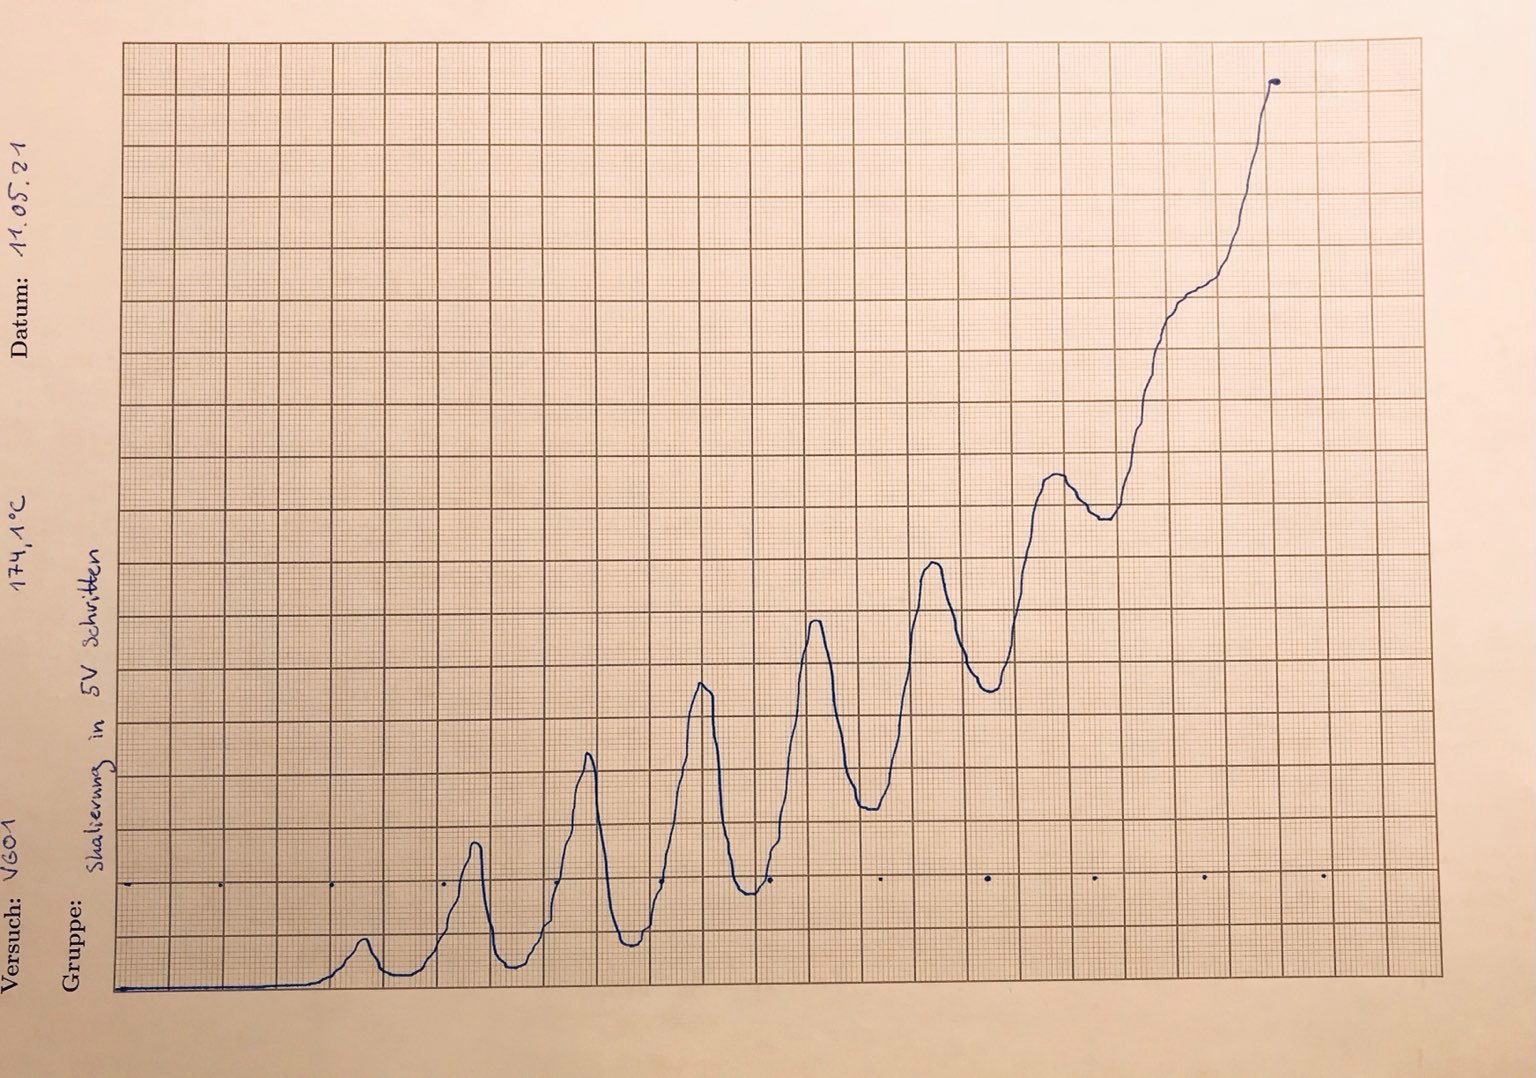
\includegraphics[scale=0.25]{content/kurv3.jpeg}
  \caption{Die Aufnahme der Franck-Hertz Kurve aus dem ersten Messdurchgang.}
  \label{fig:franckhertz1}
\end{figure}
\begin{figure}[H]
  \centering
  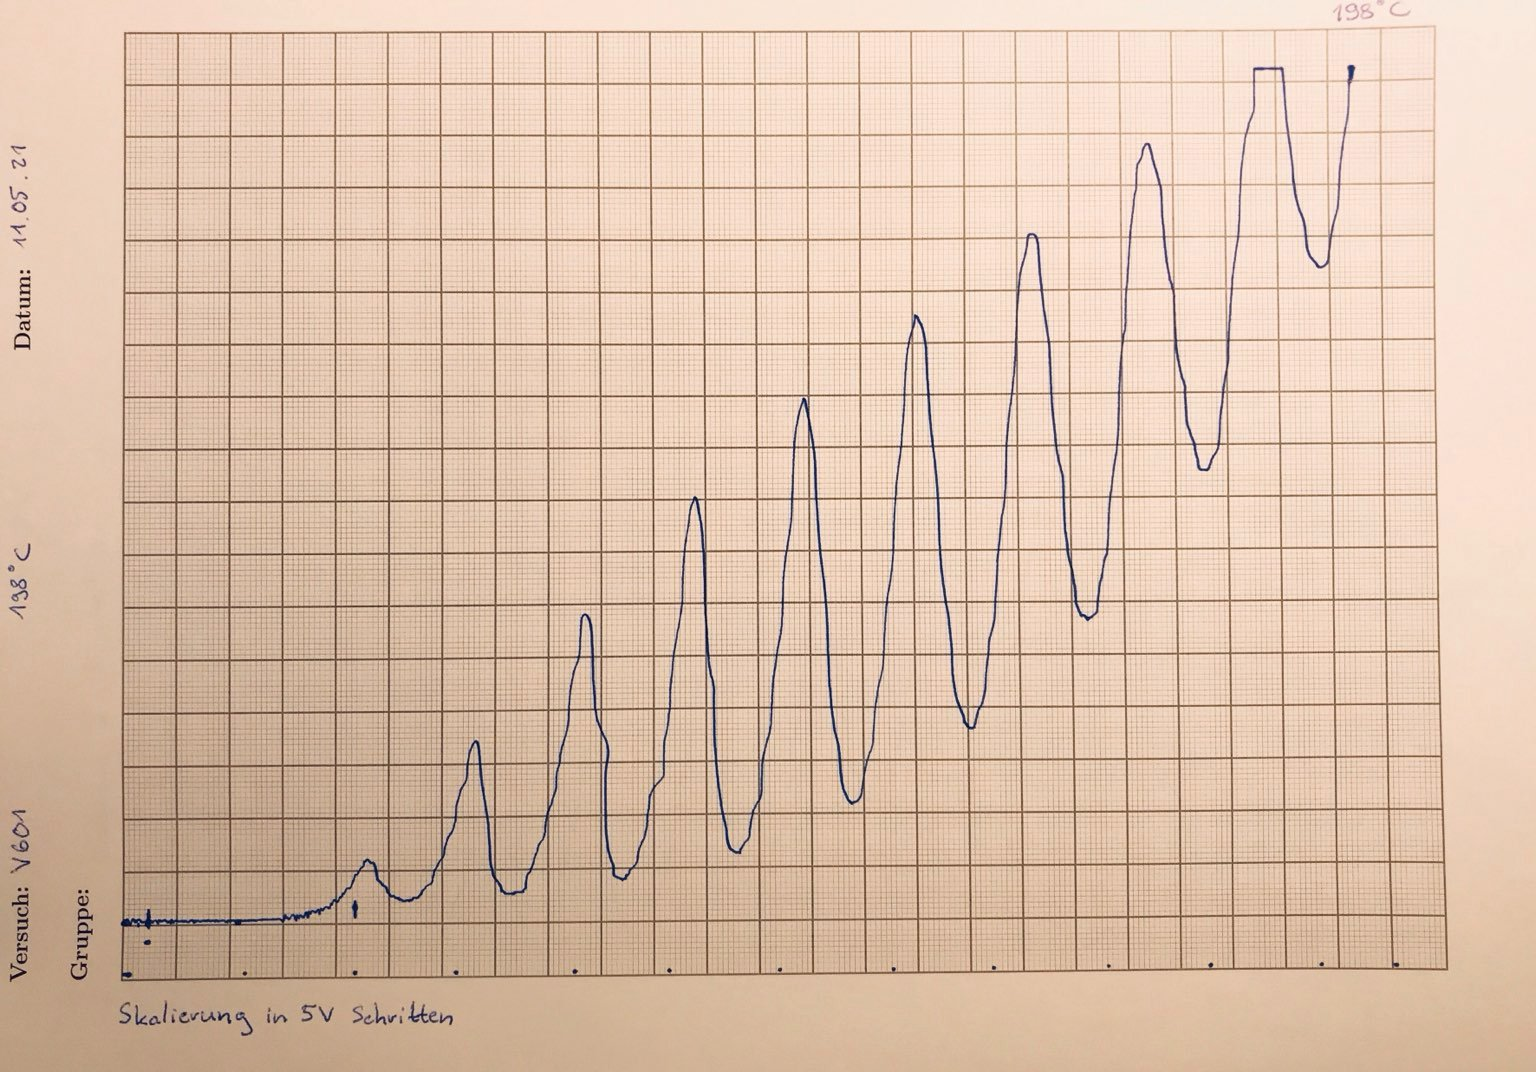
\includegraphics[scale=0.25]{content/kurve4.jpeg}
  \caption{Die Aufnahme der Franck-Hertz Kurve im zweiten Messdurchgang.}
  \label{fig:franckhertz2}
\end{figure}
